\newcommand{\todoNK}[1]{\textbf{\textcolor{red}{NK: #1}}}
\chapter{Background}
\label{chapter:background}
\newtheorem{theorem}{Theorem}
In this chapter we present the necessary background that the reader should have in order to proceed through the next two chapters, which are the core of this work. After a brief overview of kernel methods in machine learning, we will present random features and graph kernels. In the next chapter, these different notions will be combined in the proposed algorithm.

\section{Kernel methods and random features}

We first start by an overview of kernel methods.

\subsection{Kernel methods and kernel trick}
Kernel methods is a family of classic algorithms in machine learning that learn models as a combination of similarity functions between data points $(x,x')$, defined by positive semi-definite (psd) \emph{kernels} $\mathcal{K}(x,x')$. Denote by $\mathcal{D}$ the set of all possible data points. A symmetric function $\mathcal{K}:\mathcal{D}\times\mathcal{D}\mapsto\mathbb{R}$ is said to be a positive semi-definite kernel if:
\begin{equation}
\forall n\in \mathbb{N},~\forall \alpha_1,\ldots,\alpha_n\in \mathbb{R},~\forall x_1,\ldots,x_n\in \mathcal{D},\quad \sum_{i,j}^n\alpha_i\alpha_j\mathcal{K}(x_i,x_j)\geq 0 \, .
\end{equation}
\nt{Can we \emph{not} use mathcal for a function? I suggest $\kappa$}

Let us now illustrate how kernels can be incorporated to learning models and how that is useful to learn more complex functions. To do that let us consider a simple classification problem: take $\mathcal{D}=\mathbb{R}^d; d\in\mathbb{N}$, and let $(\mathbf{X},\mathbf{Y})$ be a labeled dataset of size $n$ with datapoints $\mathbf{X}\in \mathbb{R}^{n\times d} $ and labels $\mathbf{Y}\in \{-1,1\}^n$. \nt{and here $X$ and $Y$ should be mathcal right? Ok, I'll stop here for notation comments as I recall you were saying that you had not changed notations yet. Also I guess you'll need to define the vector $\mathbf{y}$ where $y_i$ is the label of $\mathbf{x}_i$} Many of the learning models designed to solve this problem, like Support Vector Machine (SVM) \nt{add ref} and Perceptron binary classifier \nt{add ref}, rely on the inner product as a measure of similarity between data points: during the training, they only use inner products $\mathbf{x}_i^T \mathbf{x}_j$, and then produce models with the following form \citep{inner_product}:
\begin{equation}
\label{eq:inner_product}
 \hat{y}(\mathbf{x})=\text{sign}\left\{\sum_{i=1}^n\alpha_iy_i\mathbf{x}_i^T\mathbf{x}\right\} \text{ with } \alpha_i\in \mathbb{R}
\end{equation}
where the values $[\alpha_i]_{i=1}^n$ in Eq. \ref{eq:inner_product} are optimized based on the dataset $(\mathbf{X,Y})$ by the learning algorithm. The intuition behind Eq. \ref{eq:inner_product} is that the output class for every new data point $x$ is expected to be the same class of nearby points in the input set $\mathcal{D}$. This is achieved by introducing the inner product $\mathbf{x}_i^T\mathbf{x}$ to control how much the class $y_i$ contributes in the output $\hat{y}(\mathbf{x})$. The parameters $[\alpha_i]_{i=1}^n$ controls how strongly the data point $x_i$ can affect other neighboring points. They mainly depend on how both classes are distributed in the input set $\mathcal{D}$, and on how much the dataset $(\mathbf{X,Y})$ is noisy. 

\begin{figure}[H]
\centering
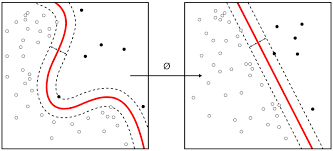
\includegraphics[scale=0.5]{figs/svm.png}
\caption[The case where classes aren't separable using linear boundary]{The left figure shows a case where the input data in their original space are not separable by a linear boundary. The right figure shows the same data transformed to a new space using a lifting function \o, and we can see that different classes are now separable  using linear boundary.}
%Source:
\label{fig:SVM_boundaries}
\end{figure}

A \emph{kernel method} consists in replacing every inner products $\mathbf{x}_i^T \mathbf{x}_j$ by a psd kernel $\mathcal{K}(\mathbf{x}_i, \mathbf{x}_j)$ during training, and similarly $\mathbf{x}_i^T\mathbf{x}$ by $\mathcal{K}(\mathbf{x}_i, \mathbf{x})$ during prediction.
Let us now explain the intuition behind this, starting by rewriting Eq. \ref{eq:inner_product} as 
\[
\hat{y}(\mathbf{x})=\text{sign}\{\textbf{x}^T(\mathbf{X}^T~diag([\alpha]_{i=1}^n)~\mathbf{Y})\},
\]
where $diag([\alpha]_{i=1}^n)$ is the diagonal matrix with values $[\alpha]_{i=1}^n$. \nt{**As $\mathbf{Y}$ is not really well defined, the reader, as it is, does not really understand the algebraic calculus at stake here**}

To get the decision boundary of such models we solve $\textbf{x}^T\textbf{q}=0$, where $\textbf{q}=(\mathbf{X}^T~diag([\alpha]_{i=1}^n)~\mathbf{Y})\in\mathbb{R}^d$. It is the equation of a hyper-plane in the input space $\mathbb{R}^d$, also referred to as a \emph{linear} decision boundary. 
The question here is: what if the the two classes are not separable by a hyper-plane (Fig. \ref{fig:SVM_boundaries})? 

One common solution to this problem is to map the data points from $\mathbb{R}^d$ to another space $\mathbb{R}^m$  through a proper mapping function \o~such \todoNK{Not fond of \o. How about $\varphi$ ?} \nt{I agree: $\varphi, \psi$?} that the two classes become separable with a linear decision boundary in $\mathbb{R}^m$. Then we can apply the same learning models specified in Eq. \ref{eq:inner_product} but on the transformed data. Let us consider for example the dataset shown in Fig. \ref{fig:polynomial_kernel},  we can use the following mapping function \o$:(x_1,x_2)\mapsto (\sqrt{2}x_1x_2,x_1^2,x_2^2)$ to move from $\mathbb{R}^2$ on the left, where data are not linearly separable, to $\mathbb{R}^3$ on the right, where they are.
\begin{figure}[H]
\centering
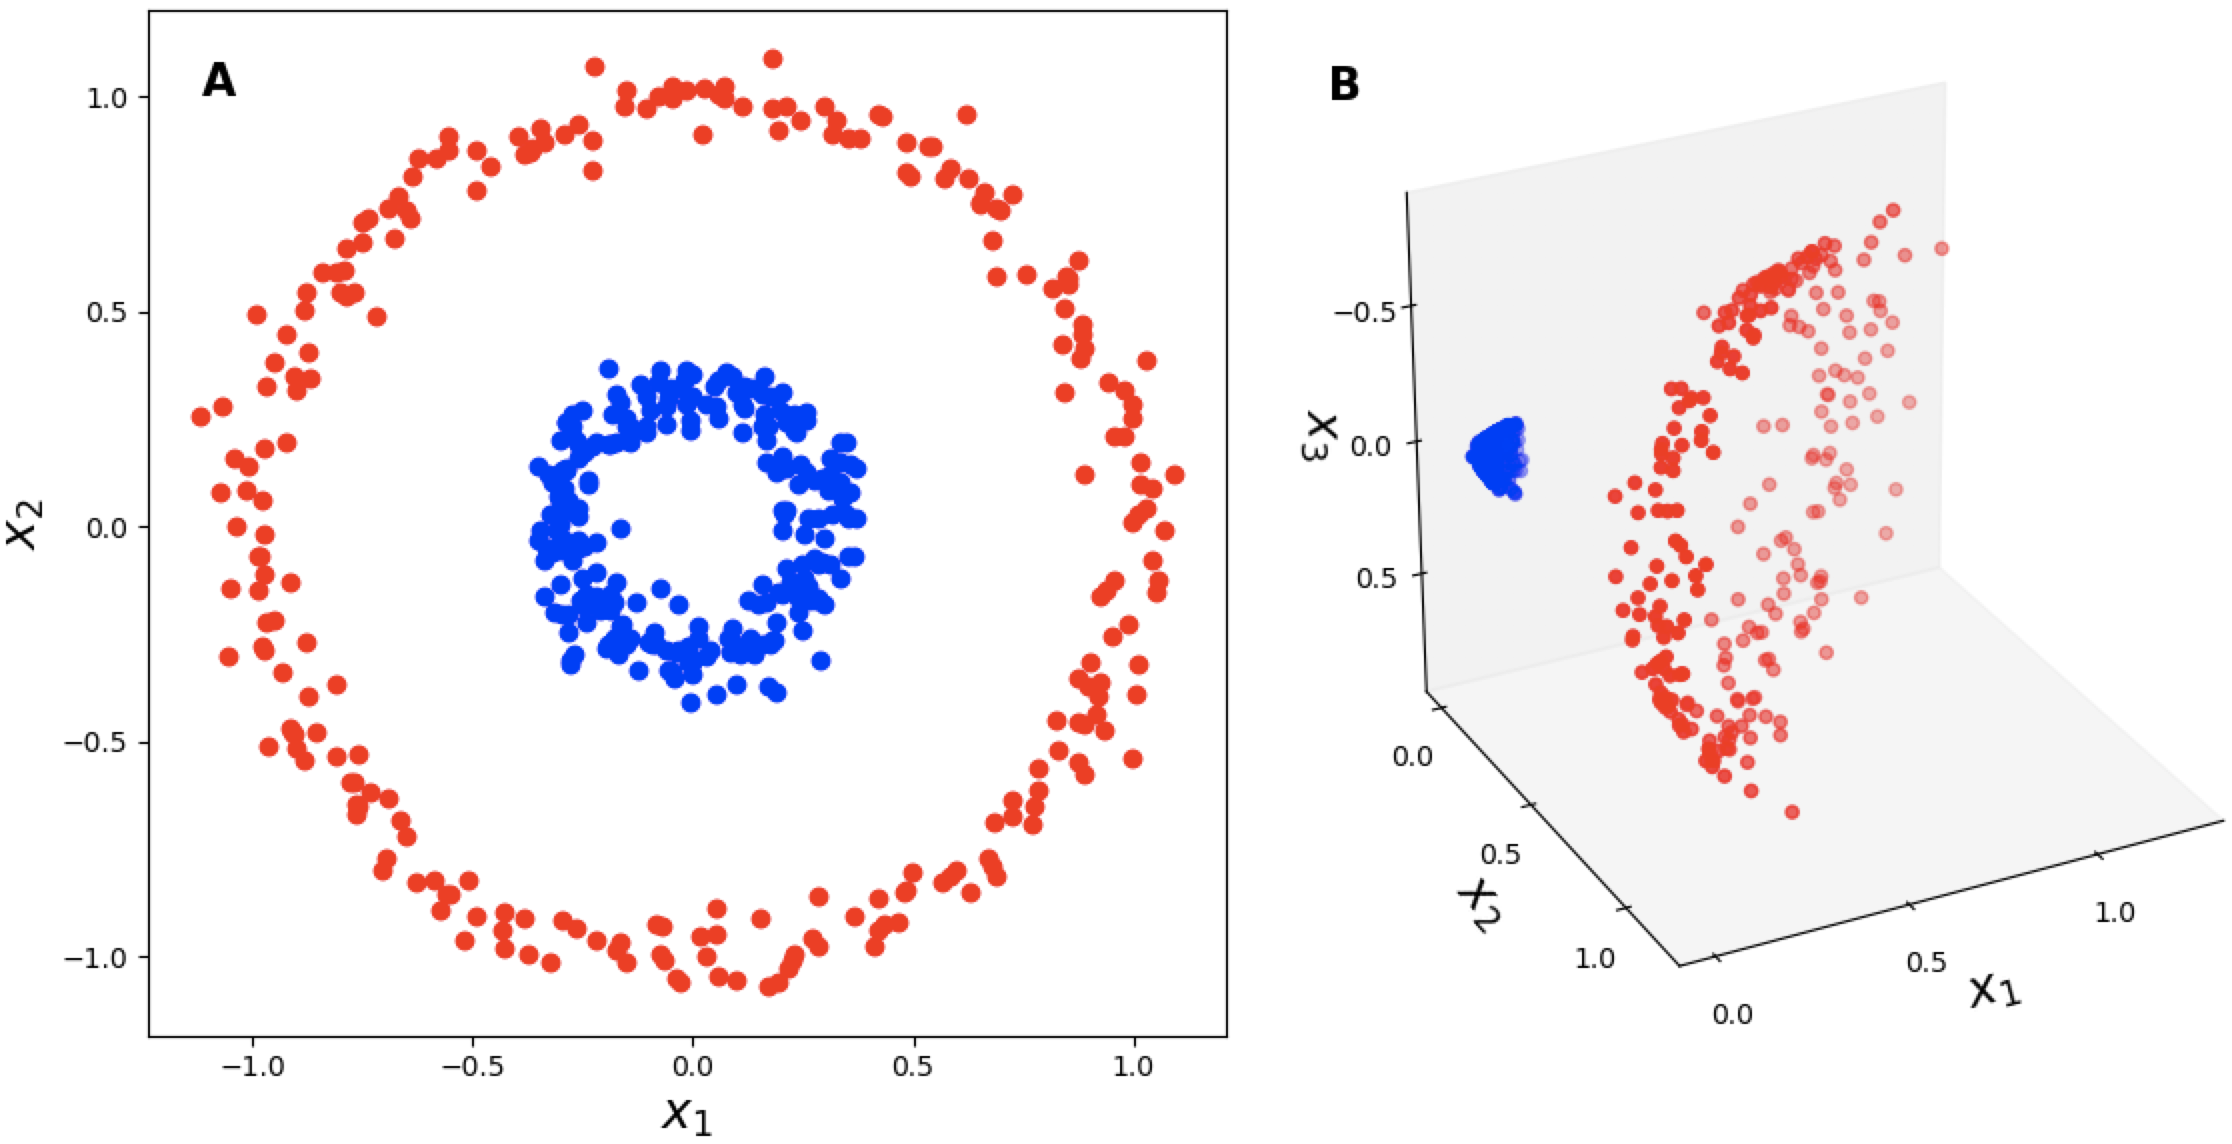
\includegraphics[scale=0.25]{figs/poly_kenrnel.png}
\caption[Lifting data to a higher-dimension space to get linearly separable classes]{ Using the mapping function \o$:(x_1,x_2)\mapsto (\sqrt{2}x_1x_2,x_1^2,x_2^2)$ to map the data on the left in $\mathbb{R}^2$ to $\mathbb{R}^3$ where they are linearly separable}
%Source:
\label{fig:polynomial_kernel}
\end{figure}
Learning such a function \o~is what is typically done by neural networks using complex optimization methods.  Kernel methods are much simpler (and elegant) methods to perform this mapping. They are justified by the following key theorem.
\begin{theorem}[Mercer theorem]
To every positive semi-definite kernel $\mathcal{K}:\mathbb{R}^d\times \mathbb{R}^d\mapsto \mathbb{R}$, there exists a Hilbert space $\mathbb{H}$ and a feature map $\phi:\mathbb{R}^d\mapsto\mathbb{H}$ such that for all $x,x'\in\mathbb{R}^d$ we have: 
\begin{equation}
\label{eq:kernel_main_equation}
    \mathcal{K}(\mathbf{x},\mathbf{x}')=<\phi(\mathbf{x}),\phi(\mathbf{x}')>_\mathbb{H}
\end{equation}
where $<\phi(\mathbf{x}),\phi(\mathbf{x}')>_\mathbb{H}$ is the inner product defined in $\mathbb{H}$.
\end{theorem}
This theorem states that replacing the inner product $\mathbf{x}_i^T\mathbf{x}$ in Eq. \ref{eq:inner_product} by a positive semi-definite kernel $\mathcal{K}(\mathbf{x}_i,\mathbf{x})$ is equivalent to implicitly map the data from the original input space $\mathcal{D}$ to another feature space $\mathbb{H}$ and then apply the classical inner product. Therefore, one \emph{does not need to know explicitely the mapping} $\phi$ nor the new feature space $\mathbb{H}$, instead, it is sufficient to evaluate the kernel $\mathcal{K}$ for pairs of data points in the original input space $\mathcal{D}$. This main feature of kernel methods is known as the \emph{kernel trick}. It has two main advantages:
\begin{itemize}
    \item Kernels allow us to transform data to a new Hilbert space of very high or even infinite dimensionality, which can make the learning model able to represent more complex functions.
    \item Kernels are often computationally cheaper, since they save the time required to compute the explicit co-ordinates of the data in the new feature space by directly calculating the inner product between the transformed data.
\end{itemize}
To better illustrate these benefits, we take the Gaussian kernel as an example, which is one of the most classical kernels in $\mathbb{R}^d$, defined as:
\begin{equation}
\label{eq:Guassian_kernel}
    \mathcal{K}_{G}(\mathbf{x},\mathbf{x}')=\exp^{-\frac{\left \| \mathbf{x}-\mathbf{x}'\right\|^2}{2\sigma^2}}
\end{equation}
where $\sigma>0$ is called the bandwidth parameter of the kernel. The lifting function $\phi_G$ of this kernel is located in a Hilbert space of infinite dimension, but the kernel can be easily evaluated for any pair $(\mathbf{x},\mathbf{x}')\in \mathcal{D}=\mathbb{R}^d$.

Despite their advantages, kernel methods still have some drawbacks:
\begin{itemize}
    \item Since for most kernels we need to evaluate the kernel on each pairs of data points, for a dataset $(\mathbf{X},\mathbf{X})$ \nt{?} of size $n$, we need $O(n^2)$ memory entries to compute what is called a Gram matrix, whose $(i,j)_{th}$ entry equals the kernel between points $\mathcal{K}(\mathbf{x_i}, \mathbf{x_j})$.
    \item Even if most kernels are designed so that they can be evaluated in polynomial time in the dimensionality of the input space $\mathcal{D}$ (for instance computing $\mathcal{K}_{G}(\mathbf{x},\mathbf{x}')$ for two vectors in $\mathbb{R}^d$ costs $d$ operations),  some kernels (especially on graphs) are computationally expensive \citep{graphlet_kernel}. \todoNK{I would not mention that here, since handling exponential computation of *each individual evaluation* of the kernel with RF is precisely what we do which has not been done before. Only the Gram matrix problem is mentioned in the original RF paper.}
\end{itemize}
To overcome these disadvantages, random feature projections is a technique developed to approximate kernels, often requiring less computational time and less memory storage.

\subsection{Random features}
Random features (RF) \citep{rahimi2008random} is an approach developed to approximate kernel methods with reduced computational time. The idea is that, instead of considering the true lifting function $\phi$ in Eq. \ref{eq:kernel_main_equation}, we explicitly map the data points using an appropriate randomized feature map $\varphi:\mathcal{D} \xrightarrow{}\mathbb{C}^m$, such that the kernel evaluated for two data points $x, x'$ is approximated by the inner product of their random features with high probability:
\begin{equation}
\label{eq:approx_RF}
\mathcal{K}(x,x')=<\phi(x),\phi(x')>_\mathbb{H} \approx \varphi(x)^*\varphi(x')
\end{equation}
Considering this approximation, we can transform the input with $\varphi$ and then apply a linear learning method as in Eq. \ref{eq:inner_product} to have a similar learning power as the original non-linear kernel machine, while often avoiding the cost of explicitly constructing the Gram matrix. Note that with RF we do not use the kernel trick anymore, but construct an explicit mapping $\varphi$ to approximate the kernel $\mathcal{K}$.

Most RF constructions are known as Random \emph{Fourier} Features (RFF), and are based on the following theorem.
\begin{theorem}[Bochner's theorem]
A continuous and shift-invariant kernel $\mathcal{K}(x,x')=\mathcal{K}(x-x')$ on $\mathbb{R}^d$ is positive definite if and only if $\mathcal{K}$ is the Fourier transform of a non-negative measure.
\end{theorem}
As a direct consequence, we can easily scale any shift-invariant kernel to obtain $\mathcal{K}(0) = \int p = 1$, so that its Fourier transform $p(w)$ is a correct probability distribution. We obtain that any shift-invariant psd kernel is of the form:
\begin{equation}
\label{Fourier integral}
\mathcal{K}(x-x')=\int_{\mathbb{R}^d}p(w)e^{jw^T(x-x')}dw= E_w[\xi_w(x)^*\xi_w(x')]
\end{equation}
where $\xi_w(x)=e^{-jw^Tx}$, where the expectation $E_w$ is over the appropriate probability distribution $p(w)$. Note that, since $\mathcal{K}$ is a real-valued function, from Eq.~\ref{Fourier integral} one can also prove that:
\begin{equation}
\label{real Fourier integral}
\mathcal{K}(x-x')=\int_{\mathbb{R}^d}p(w)cos({w^T(x-x')})dw=E_w[\tilde \xi_w(x)\tilde \xi_w(x')]
\end{equation}
where $\tilde \xi_w(x)=\sqrt{2}cos(w^Tx+b)$ such that $w$ is drawn from $p(w)$ and b is drawn uniformly from $[0,2\pi]$, so we can use real-valued mapping if desired.

As a result, for $w$ a random variable drawn from $p(w)$, $\ \xi_w(x)\xi_w(x')$ is an unbiased estimate of $\mathcal{K}(x,x')$. The RF methodology consists in averaging $m$ instances of the estimator with different random frequencies $w_j$ drawn identically and independently (iid) from $p(w)$, that is, define
\[
\varphi(x) = \frac{1}{\sqrt{m}} ( \xi_{w_j}(x) )_{j=1}^m \in \mathbb{C}^m
\]
such that $\varphi(x)^*\varphi(x')=\frac{1}{m} \sum_{j=1}^m \xi_{w_j}(x)^*\xi_{w_j}(x')$, which converges to $\mathcal{K}(x,x')$ by the law of large numbers. Moreover, Hoeffding's inequality guarantees exponentially fast convergence in $m$ between $\varphi(x)^*\varphi(x')$ and the kernel true value:
\begin{equation}
   \forall \epsilon >0\qquad Pr(|\varphi(x)^*\varphi(x')-\mathcal{K}(x,x')|\geq\epsilon)\leq2e^\frac{-m\epsilon^2}{4},
\end{equation}
that is, for any error $\epsilon$, the probability that the estimation is off by more than $\epsilon$ is controlled by an exponentially decaying term.

\nt{I would add here the theorem of the form (the union bound on the previous Hoeffding):
\begin{theorem}\label{thm:RF_vs_logn}
Let $\epsilon\in(0,1)$ and $\delta\in(0,1)$. Consider a dataset $\mathcal{X}=(\mathbf{x}_1,\ldots,\mathbf{x}_n)$ of $n$ elements, and a psd shift-invariant kernel $\kappa$. The random embedding  $\varphi(x)\in\mathbb{R}^m$ enables a controlled approximation of \emph{all} the elements of the Gram matrix with probability larger than $1-\delta$, \emph{i.e.}
$$\text{Pr}\left(\forall (\mathbf{x}, \mathbf{x}')\in\mathcal{X}^2\quad|\varphi(x)^*\varphi(x')-\mathcal{K}(x,x')|\leq\epsilon\right)\geq 1-\delta$$ 
provided that 
$$m\geq\mathcal{O}\left(\frac{1}{\epsilon^2}\log{\frac{n}{\delta}}\right).$$
\end{theorem}
I find this version useful as we clearly see that in fact random embedding is classically useful when $\log{n}\leq d$. If $d$ is too small, random embedding is in general useless. }

As an illustration, consider the Gaussian kernel in Eq. \ref{eq:Guassian_kernel} as an example. This kernel is shift-invariant and known to be positive semi-definite. It is already correctly normalized since $\mathcal{K}(0) = 1$, and its Fourier transform is a Gaussian probability distribution with inverted variance:
\[p(w)=FT\big(\mathcal{K}_G\big)(w)=\left(\frac{\sigma^2}{2\pi}\right)^\frac{d}{2}e^{-\frac{\sigma^2\|w\|^2}{2}}\]
Thus, in practice, in order to approximate the Gram matrix of $\mathcal{K}_G$ on a dataset $\mathcal{X}$ of size $n$, one i/~draws $m$ iid frequencies from this probability distribution, with $m$ as in Theorem~\ref{thm:RF_vs_logn}; ii/~uses these frequencies to associate to each element $x\in\mathcal{X}$ its associated random feature vector $\varphi(x)\in\mathbb{R}^m$; iii/~uses $\varphi(x)^*\varphi(x')$ as an approximation of $\kappa_G(\mathbf{x},\mathbf{x}')$ where necessary in any kernel-based learning algorithms.

\section{Graphlet kernel}
Kernel methods are a flexible set of tools, since psd kernels can be defined on any set of objects rather than on vectors $x\in \R^d, d\in \mathbb{N}$ \nt{*which should be $\mathbf{x}\in \R^d, d\in \mathbb{N}$}. Naturally, for machine learning tasks on graphs such as graph classification or regression, authors have developed kernels on graphs $\mathcal{K}(G,G')$ \nt{*which should be $\kappa(\mathcal{G},\mathcal{G}')$} \citep{kriege_graph_kernels}. This section gives a brief overview of graph kernels, focusing on the so-called \emph{graphlet kernel}, which will be our main inspiration for this work. We start with a few definitions.
\subsection{Notations of graphs and graphlets}
Recall that a graph $\mathcal{G} = (\mathcal{V}, \mathcal{E})$ is formed by a set of nodes and a set of edges connecting them. A graph $F=(\mathcal{V}_F,\mathcal{E}_F)$ is said to be a subgraph (also called \emph{graphlet}) of $\mathcal{G}$, written $F\sqsubseteq \mathcal{G}$, if and only if there exists an injective function $\mathcal{M}:\mathcal{V}_F\xrightarrow{} \mathcal{V}$ such that $(u,u')\in \mathcal{E}_F \Leftrightarrow{(\mathcal{M}(u),\mathcal{M}(u'))\in \mathcal{E}}$.

Any edge $(u_i, u_i)$ is called a self loop. In a general graph two vertices $u_i$ and $u_j$ may be connected by more than
one edge. A simple graph is a graph with no self loops or multiple edges. Here we always consider simple graphs.
A (simple) graph can equivalently be represented by an adjacency matrix $\mathbf{A}$ of size $v \times v$. The $(i,j)-th$ entry of $\mathbf{A}$ is 1 if an edge $(u_i, u_j)$ exists and zero otherwise.

Two graphs $\mathcal{G}=(\mathcal{V},\mathcal{E})$ and $\mathcal{G'}=(\mathcal{V'},\mathcal{E'})$ are said to be \emph{isomorphic}, written $\mathcal{G}'\cong \mathcal{G}$, if there exists a bijective function $\mathcal{M}:\mathcal{V}\xrightarrow{} \mathcal{V}'$ such that $(u_i,u_j)\in \mathcal{E}$ iff $(\mathcal{M}(u_i),\mathcal{M}(u_j))\in \mathcal{E}'$. Deciding if two graphs are isomorphic is known to be a difficult problem: it is actually an open question if this problem is solvable in polynomial time or is NP-complete. It is equivalent to test if two adjacency matrices are a permutation of each other. This gives us a clue why the isomorphism test is expensive: in the worst case where the graphs to be compared don't have a specific structure which can used as \emph{a prior}, the brute force method considers all the $v!$ permutation matrices. There are efficient, specific methods for small graphs \citep{graphlet_kernel}, but the general case is still open. We denote by $C_k$ the computational cost of testing the isomorphism between two graphs of size $k$. \nt{I sort of remember we had decided upon $C^{\cong}_k$ for the cost of isomorphic testing of size $k$. But perhaps $\cong$ is not needed if we don't need $C_k$ somewhere else.}

As we will see, for a given graph, the graphlet kernel is defined by counting small subgraphs of size $k$, also called graphlets. We introduce some convenient notations. Let us denote by $\mathfrak{H}=\{\mathcal{H}_1,..., \mathcal{H}_{N_k}\}$ the set of all possible graphlets of size $k$. Depending on the context, there is two choices in defining this set. Either we count all possible adjacency matrices and treat isomorphic graphs as different graphs, in which case we have $N_k=2^{k(k-1)/2}$ different graphlets. We refer to this set as the set of graphlets \emph{with repetition}. Or we do not distinguish isomorphic graphs, so we have here $N_k<2^{k(k-1)/2}$ but it is still exponential in $k$. We call this set the set of graphlets \emph{without repetition}. The classical graphlet kernel uses graphlets without repetition, which can require expensive isomorphism tests. We will see that some methods on graphlets \emph{with} repetition also perform well in practice.

Say we sample a graphlet $F$ \nt{*should be $\mathcal{F}$*} of size $k$ from a given graph $\mathcal{G}$. A possibly expensive operation is to find, in the list of all possible graphlets of size $k$, $\mathfrak{H}_k$, which one it matches. We define the matching function $\varphi_{k}^{match}$, which, in the case of graphlets with repetition is defined as: 
\[
\varphi_k^{match}(F) = \left[ 1_{(F = \phlet_i)}\right]_{i=1}^{N_k}= \left[ 1_{(\mathbf{A}_F = \mathbf{A}_{\phlet_i})}\right]_{i=1}^{N_k} \in \{0,1\}^{N_k}
\]
\nt{$\varphi$ should be bold, as it is a vector}
In words, $\varphi_k^{match}$ is a Boolean vector of dimension $N_k$ and has a $1$ in the coordinate $i$ if the adjacency matrices of both graphs $F$ and $\phlet_i$ are equal, and $0$ otherwise. Clearly the cost of each test is $k^2$, and the global cost of applying $\varphi^{match}_k$ is $O(N_k k^2)$. On the other hand, when the case of graphlets \emph{without repetition} is considered, $\varphi_k^{match}$ is defined as:
\[
\varphi_k^{match}(F) = \left[ 1_{(F \cong \phlet_i)}\right]_{i=1}^{N_k} \in \{0,1\}^{N_k}
\]
which means that $\varphi_k^{match}$ puts a $1$ in the coordinate $i$ if $F\cong \phlet_i$, and $0$ otherwise. The global cost is now $O(N_k C_k)$, with an isomorphic test cost $C_k$ potentially exponential in $k$ thus much larger than $k^2$, although for a $N_k$ smaller than the case with repetition.  

Let $\mathfrak{F}=\{\mathcal{F}_1,\ldots,\mathcal{F}_s\}$ be a set of $s$ size-$k$ graphs. We define the function $\varphi_k^{hist}$ which counts, for each graphlet $\phlet_i$ in $\mathfrak{H}$, how many matches it has in $\mathfrak{F}$. Here we use either version of $\varphi_k^{match}$, and write:
\[
\varphi_k^{hist}(\mathfrak{F})=\frac{1}{s}\sum_{\mathcal{F}\in\mathfrak{F}} \varphi_k^{match} (\mathcal{F}) \in \R^{N_k}
\]
\nt{$\varphi$ should be bold}
where the term $\frac{1}{s}$ is introduced for normalization purposes in order for  $\varphi_k^{hist}(\mathfrak{F})$ to sum to 1. %With this definition and when $s$ is sufficiently large, $\varphi_k^{hist}(\mathbf{F}_\G)$ can be seen as the vector whose $i_{th}$ entry has the frequency of graphlet $\phlet_i$ in the graph $\G$.


\subsection{Convolutional graph kernels}
Recall that traditional kernel machines are applied to problems with vector-valued input data, where they compare different data points $x,x' \in \mathcal{R}^d$, \nt{what is $\mathcal{R}$?} often through their Euclidean distance. Based on that, these kernels cannot be used directly on (a vector representation of the) graphs: indeed, isomorphic graphs have different adjacency matrices representing the same structure. As a result it is necessary to measure distances between graphs in ways that are insensitive to isomorphism: ideally, if $\mathcal{G}_1 \cong \mathcal{G}'_1$ and $\mathcal{G}_2 \cong \mathcal{G}'_2$, then $\mathcal{K}(\mathcal{G}_1, \mathcal{G}_2)$ should be equal to, or at least very close to, $\mathcal{K}(\mathcal{G}_1', \mathcal{G}_2')$. One observes that the concept of isomorphism is critical in learning algorithms on graphs, not only because there is no known polynomial-time algorithm for testing graph isomorphism (except for graphs with specific structures), but simply testing isomorphism is also too strict for learning in a similar way to learning with equality operator \nt{not able to re-write this last sentence: I do not understand it} \citep{kriege_graph_kernels}.

Since it is simpler to define kernels on \emph{small} graphs (as testing isomorphism is computationally feasible for small graphs), most of the graph kernels in the literature belong to the family of \emph{convolution kernels}: given two graphs, the trick is to divide each into smaller subgraphs and then to pairwise compute a kernel between the resulting subgraphs.
\newtheorem{definition}{Definition} 
\begin{definition}[Convolution Kernel]
let $\mathcal{R}=\mathcal{R}_1\times...\times \mathcal{R}_d$ denote a space of components such that a composite object $X\in \mathcal{X}$ decomposes into elements of $\mathcal{R}$. Let $R:\mathcal{R}\xrightarrow{}\mathcal{X}$ denote the mapping from components to objects, such that $R(x)=X$ iff the components $x\in \mathcal{R}$ make up the object $X\in \mathcal{X}$, and let $R^{-1}(X)=\{x\in\mathcal{R}:R(x)=X\}$. then, the R-convolution kernel is:
\begin{equation}
\label{eq:conolutional_kernels}
    K_{CV}(X,Y)=\sum_{x\in R^{-1}(X)}~\sum_{y\in R^{-1}(Y)}~\underbrace{\prod_{i=1}^{d}k_i(x_i,y_i)}_{k(x,y)}
\end{equation}
with $k_i$ is a kernel on $\mathcal{R}$ for $i\in\{1,...,d\}$.
\end{definition}
\nt{**I think we should re-write this definition directly in the graph context. This component/object thing is too abstract in the current flow of discussion**}
\nt{**Also, can we use a small latin letter for the function $R$?**}

Applying this definition on graphs, $R^{-1}(\mathcal{G}=(\mathcal{V},\mathcal{E}))$ includes all the components in graph $\mathcal{G}$  that we want to compare with the components $R^{-1}(\mathcal{G'}=(\mathcal{V}',\mathcal{E}'))$ in graph $\mathcal{G'}$. One example of these kernels is the node label kernel, where for two graphs $\mathcal{G}, \mathcal{G'}$, the mapping function $R$ maps the features $x_u\in \mathcal{R}$ of each node $u\in \mathcal{V}\cup \mathcal{V'}$ to the graph that $u$ is a member of. \nt{I understand this last sentence, but I think it is incomplete for the reader. Ok you have such a function, but what happens then? Explain briefly what $\kappa_{CV}$ actually does in this case, which could perhaps motivate the following choice of graphlet kernel.} Another example, which will be our main source of inspiration and will be further described in the next section, is the $k$-graphlet kernel, where $R$ here maps the subgraphs of size $k$ to the graph in which they occur.
 
The advantage of using the convolution kernel framework with graphs is that kernels are permutation invariant, non-sensitive to  on the graphs level as long as they are permutation invariant on the components level \nt{this last sentence lacks words to be understandable}. As a drawback, the sum in Eq.~\ref{eq:conolutional_kernels} iterates over every possible pair of components. As a result, when the base kernel has high value between a component and itself while it is low between two different components, each graph becomes drastically similar to itself but distant from any other graph. Thus, a set of weights is usually added to counter-balance this problem.

\subsection{Graphlet Kernel}
\label{subsection: graphlet kernel}

As mentioned above, the graphlet kernel is a special instance of convolution kernel equivalently described as follows: one enumerates all the subgraphs of size $k$ of each graph (where $k$ is small), counts them to build a histogram of their frequencies of apparition, and takes the inner product between the two histograms to obtain the final kernel. In this context, the subgraphs are called ``graphlets'', as an analogy with classical wavelets, which are individual components of more traditional signals.

For a graph $\mathcal{G}=(\V,\E)$, we define the vector $f_\mathcal{G}\in \mathcal{R}^{N_k}$ \nt{you mean $\mathbb{R}^{N_k}$? + we actually don't define $\mathbf{f}_\mathcal{G}$ here: it was already defined} whose $i$-th entry equals the normalized-number of occurrences of $\mathcal{H}_i$ in $\mathcal{G}$, usually referred to as the $k$-spectrum of $\G$. In details, defining $\mathfrak{F}_\G=\{F_1,\ldots,F_s\}$ the set of \emph{all} size-$k$ subgraphs in $\G$, that is, $s=\tbinom{v}{k}$ for graphlets without repetition \nt{with this choice of $s$, this is the case \emph{with} repetition! + let's not use $s$ here as it will be a number of samples afterwards..}. We have:
\[
\mathbf{f}_\G=\bm{\varphi}_k^{hist}(\mathfrak{F}_\G) \in\mathbb{R}^{N_k}
\]
\nt{Conveniently, $\bm{\varphi}_k^{\rm hist}$ is already defined: let's call it to start making connections between the different parts of the report.}
where graphlets are considered without repetition. The graphlet kernel is then the inner product between the histograms.
\begin{definition}[Graphlet Kernel]
Given two graphs $\mathcal{G}$ and $\mathcal{G}'$ of size $\geq k$, the graphlet kernel $\kappa$ is defined as \citep{graphlet_kernel}:
\begin{equation}
\label{eq:graphlet_kernel}
    \kappa(\mathcal{G},\mathcal{G}')=\mathbf{f}_{\mathcal{G}}^T \mathbf{f}_{\mathcal{G}'}.
\end{equation}
\end{definition}
\nt{I dropped the sub-g in $\kappa_g$ for ease of notation}
In this case the distance between graphs in the kernel space is just the Euclidean metric between histograms $d_\kappa({\mathcal{G}},{\mathcal{G}'}) = \|\mathbf{f}_{\mathcal{G}} - \mathbf{f}_{{\mathcal{G}'}}\|_2$. Also, from now on, unless otherwise specified, $\kappa$ will refer to this graphlet kernel. 

\textbf{The computational cost} is a major drawback of this kernel, as computing the $k$-spectrum vector $\mathbf{f}_{\mathcal{G}}$ is very costly, even for moderate $k$: there are $\mathcal{O}\tbinom{v}{k}$ subgraphs of size $k$ in a graph of size $v$, the number of graphlets of size $k$, $N_k$, is exponential in $k$, and since graphlets are taken without repetition multiple isomorphism tests must be performed. Thus, this cost can be written as:
\begin{equation}
\label{eq:cost_graphlet}
    C_{gk}= \mathcal{O}(\tbinom{v}{k} N_k C_k)
\end{equation}
As a result, there is a trade-off between a more accurate representation of the graph (larger value of $k$) and the computational cost. However, some techniques are used in order to handle this limitation. In the next section, we focus on empirical sampling.

\subsection{Graph sampling to approximate k-graphlet spectrum}
\label{graph_sampling}
%Graph sampling arises when we deal with a large-scale graph and the task is to pick a small-size sample subgraph that would be similar to the original graph with respect to some important properties.

The graphlet kernel can be interpreted as follows: if one draws a subgraph randomly from $\mathcal{G}$, then one has a probability $(\mathbf{f}_\mathcal{G})_i$ of obtaining $\mathcal{H}_i$. So, it is natural to approach $\mathbf{f}_\mathcal{G}$ with an empirical histogram, built by  sampling $s$ subgraphs $\hat{\mathfrak{F}}_\G=\{\mathcal{F}_1,...,\mathcal{F}_s\} \sqsubseteq \mathcal{G}$ of size $k$, and then estimate the $k$-spectrum vector empirically: $\hat{\mathbf{f}}_\mathcal{G} =\bm{\varphi}_k^{hist}(\hat{\mathfrak{F}}_\G)= \frac{1}{s}\sum_{j=1}^s \varphi^{match}_k(F_j)$. In other words, we count the number of times $\mathcal{H}_i$ appears among the samples. The Law of Large Numbers states that $\hat{\mathbf{f}}_\G \xrightarrow[s \to \infty]{} \mathbf{f}_\mathcal{G}$ with probability $1$ \nt{**euh.. well that depends on the sampling method! For uniform random sampling yes. For the dummy sampling method that samples always $\mathcal{H}_1$, no. For the random walk sampling (even with the fly option), I believe no also.**}

This adds a degree of freedom to the method: there are many different ways of sampling a subgraph of size $k$ from a graph \citep{graph_sampling}. A \emph{sampling method} will generically be denoted by $S_k(\mathcal{G})$. We will denote by $F \sim S_k(\G)$ a random $k$-subgraph of $\G$ sampled by $S_k$. Note that each sampling method defines \emph{a different histogram} $\mathbf{f}_\mathcal{G} = \mathbb{E}_{F \sim S_k(\G)} \bm{\varphi}^{match}_k(F)$ \nt{should be called $\mathbf{f}_{S_k(\mathcal{G})}$ probably} when $s \to \infty$ \nt{**the previous definition with the expected value does not depend on $s$}. We describe two examples that we will use in the experiments.
\begin{itemize}
\item \textbf{Uniform sampling}: this is the simplest sampling method. We select a subset of $k$ nodes uniformly at random among the $\tbinom{v}{k}$ possible choices, and extract the subgraph induced by these nodes. This is the sampling method that corresponds to the classical graphlet kernel \eqref{eq:graphlet_kernel} when $s \to \infty$.
\item \textbf{Random walk sampling}: here we sample the subgraph node by node, we first randomly choose a node $u$ from $\V$ to be the starting node. Then and till we collect $k$ nodes, we choose the next node randomly from the current node's neighbors in $\G$, and with probability $p_{flyback}$ we go back to the starting node and repeat the same from there, or we stay at the recently chosen node.
\end{itemize}
The difference between the two methods is that unlike uniform sampling, random walk sampling tends \nt{**more than ``tends'', it will sample connected subgraphs no?**} to generate connected subgraphs, \emph{i.e.} there is a path of edges between any pair of the subgraph. This difference is important when we want to sample large graphs where the average number of edges incident to a node is small compared to the graph size, as uniform sampling in this case generates sparse subgraphs that don't have any edge or just few with high probability. Taking this into account, it is necessary to use random walk when possible since the frequencies of sparse graphlets is high in all the graphs and thus not discriminative to be used in a learning algorithm.

The question here is how many samples we should consider in order to have a desired certainty in our estimation, the following answer this question for every sampling technique $S_k$ whose corresponding $\varphi_k^{hist}$ converge to $f_\G$ when the number of sample grows to infinity.
%\newtheorem{theorem}{Theorem} 
\begin{theorem}
Let $f_\G$ be a probability distribution on the finite set of k-nodes graphlets  $\mathfrak{H}=\{\phlet_1,...,\phlet_{N_k}\}$, and $\mathfrak{F}=\{F_1,...,F_{s}\}$ be a set of \emph(iid) random subgraphs drawn from $f_\G$ \nt{are we doinf iid or ``any sampling technique whose corresponding $\varphi_k^{hist}$ converges to $f_\G$'' as stated above? + the subgraphs are drawn via $S_k(\G)$ not from $\mathbf{f}_\G$} . Then for a given $\epsilon>0$ and $\delta >0$ we have \citep{graphlet_kernel}:
\begin{equation}
s_{min}=\left \lceil \frac{2(log(2)N_k+log(\frac{1}{\delta} ))}{\epsilon^2} \right \rceil
\end{equation}
samples are enough to ensure that $Pr(\| f_\G-\varphi_k^{hist}(\mathbf{F}) \|_1 \geq \epsilon )\leq\delta$, where $\lceil.\rceil$ is the ceiling function. \nt{**$\varphi_k^{hist}(\mathbf{F})$ has a name**}
\end{theorem}

\textbf{The computational cost} of approximating $k$-graphlet spectrum using graph sampling %and then averaging} the matching function $\varphi_k^{match}$, will be referred to with $\mathbf{GSA}-{\varphi_k^{match}}$, 
includes the cost of sampling a single subgraph with the process $S_k$, denoted by $C_S$, iterating over all $s$ sampled subgraphs $F_j\sqsubseteq \G$, then applying $\varphi^{match}_k$ as before. So the computational cost of this method is:
\begin{equation}
\label{eq:cost_graphlet_sampling}
    C_{gk + gs}= O(C_s s N_k C_k)
\end{equation}

\todoNK{Quick comparison with the exhaustive case since the proposition above states $s \sim N_k$ ?}

